%!TEX root = ../Thesis.tex
\section{Dokumentation der Software}

\subsection{Dokumentation der Paketstruktur des Android-Projektes}

\subsection{Überblick über die Activities der App bzw. der Funktionen}

\subsection{Dokumentation der Navigation zwischen Activities}

\subsection{Dokumentation der Activity-übergreifenden, persistenten Datenhaltung}

\subsection{Dokumentation der programmatischen Beiträge der Teammitglieder}

\subsubsection{Tom Bockhorn}

\newpage

\subsubsection{Hendrik Falk}

\newpage

\subsubsection{Dennis Gentges}

\newpage

\subsubsection{Getuart Istogu}

\newpage

\subsubsection{Jannis Keienburg}

\newpage

\subsubsection{Tim Jonas Meinerzhagen}

\newpage

\subsubsection{Khang Pham}

\newpage

\subsubsection{Tim Schwenke}

\para{Generische Kalkulationsorchestrierung}

Wie schon im Kapitel zur Projektplanung erwähnt, stellt die Strukturierung und Architektur der Rechnungsumsetzung im Backend eine der vielen Anforderungen des Projekts dar. Identifiziert wurden zwei Hauptarten von Kalkulationen. 

Die erste Art ist generisch und wird in einer großen Anzahl benötigt. Ein Beispiel dafür ist die Addition. Da der Taschenrechner viele unterschiedliche Operanden-Typen unterstützt (Matrizen, Brüche, Mengen, usw.) sind enorm viele Methoden notwendig, um alle Möglichkeiten der Addition abdecken zu können. Auch muss irgendwo vom Programm entschieden werden, welche Methode genau aufgerufen werden soll. Statt dies mit komplexen If-Else-Bedingungen zu lösen, wurde in der Planungsphase entschieden Reflektion zu nutzen. Somit kann man in sich geschlossene kleine Methoden programmieren, die - sofern die Schnittstellenanforderungen erfüllt sind - automatisch erkannt und von der Reflektionsmethode aufgerufen werden können. Der Nutzer im Frontend muss lediglich entscheiden, was für eine Art von generischer Kalkulation er ausführen möchte. Zum Beispiel Addition oder Multiplikation. 

Die zweite Art von Kalkulationen sind sehr spezifisch, z.B. ein bestimmter Algorithmus zum Lösen von kubischen Gleichungen. Hier sind keine/kaum Kombinationen möglich und können somit direkt aufgerufen werden, ohne Reflektion zu verwenden.

Implementiert ist die Reflektion in der abstrakten Klasse \code{Action}. Die Klassenvariable \code{scopedAction} zeigt zur Laufzeit auf eine konkrete Implementierung einer \code{Action}, also z.B. \code{Plus}. Auf \code{scopedAction} wird die Reflektion ausgeführt. Letztere ist in der Methode \code{with()} umgesetzt. Diese stellt die Schnittstelle zu den generischen Kalkulationen erster Art dar. Hier ist der Methodenkopf zu sehen:

\begin{figure}[bht]
	\begin{lstlisting}[
	caption=Methodenkopf der generischen Schnittstelle,
	label=list:methodenkopf-der-generischen-schnittstelle,
	language=Java]
@Contract(pure = true) public @NotNull 
Operand with(@NotNull Operand... operands) 
throws CalculationException
	\end{lstlisting}    
\end{figure}

Die erste Zeile definiert einige Eigenschaften der Methode. \code{@Contract} sagt aus, dass die Funktion \textit{pure} ist. Sie gibt für Tupel von Operanden immer das gleiche Ergebnis zurück und ist grundsätzlich ohne Nebeneffekte. Das ist hilfreich für das automatische Testen. Als Parameter wird ein beliebig gro"ses Array von Operanden übergeben. Das Ergebnis ist immer eine valide Instanz von \code{Operand}. Wird versucht eine nicht unterstützte Kalkulation auszuführen, wird \code{CalculationException} geworfen. Diese Ausnahme ist keine \code{RunTimeException} und muss deswegen explizit behandelt werden. Alternativ hätte man hier auch Optionals nutzen. Jedoch unterstützt die genutzte Version der Android API dieses Java-Feature nicht.

\begin{figure}[bht]
	\begin{lstlisting}[
	caption=Implementierung der generischen Schnittstelle,
	label=list:implementierung-der-generischen-schnittstelle,
	language=Java]
Class[] operandClasses = new Class[operands.length];
Operand resultOperand;

for (int i = 0; i < operands.length; i++)
	operandClasses[i] = operands[i].getClass();

try {
	resultOperand = (Operand) scopedAction.getClass()
		.getDeclaredMethod("on", operandClasses)
		.invoke(scopedAction, (Object[]) operands);
} catch (SeveralExceptions e) {
	throw new CalculationException(e.getMessage());
}

if (resultOperand != null) return resultOperand;
else throw new CalculationException();
	\end{lstlisting}    
\end{figure}

Die Reflektion in Listing~\ref{list:implementierung-der-generischen-schnittstelle} beginnt mit der Extraktion der Klasse jedes übergebenen Operands. Das kann z.B. die Klasse \code{Matrix} oder \code{Fraction} sein, die alle von \code{Operand} erben. Die extrahierten Klassen werden in Array \code{operandClasses} gespeichert. Die hier vorliegende Sequenz liefert die Antwort auf die Frage, welche konkrete Methode aufgerufen werden soll. Die Entscheidung basiert alleine auf dieser Sequenz und der konkreten \code{Action} auf die \code{scopedAction} zeigt. Aus letzterer Variable wird die Klasse extrahiert und die Methode \code{getDeclaredMethod()} aufgerufen. Damit kann man eine Methode in einer Klasse auf Basis des Namens (in unserem Falle immer \code{on}) und eine Sequenz von Parametertypen finden. Diese wird anschlie"send mit \code{invoke()} aufgerufen, wobei die Operanden übergeben werden. Kommt es zu einem Fehler werden alle Fehlertypen in \code{CalculationException} zusammengefasst und weitergegeben. Ansonsten wird das Ergebnis zurückgegeben.

\newpage












\subsection{Beschreibung von Problemen}

\subsubsection{Softwareentwicklung im Team [Schwenke]}

Schon kurz nach der initialen Erstellung des Git-Repositories und des Projekts in Android-Studio hat sich die Frage gestellt, wie man in einem acht Mitglieder starkem Team produktiv an einer einzelnen Code-Basis arbeiten soll. Hat man ein Quellcodeverzeichnis alleine für sich reichen zumeist um die drei aktive (also nicht \textit{stale}) Branches aus. Das wäre zunächst der \code{Master}-Branche, welcher die Wurzel des Verzeichnisses darstellt und – gerade, wenn Ansätze wie CI/CD verfolgt werden – die produktiven oder zumindest lauffähigen Versionen eines Projekts enthält. Im \code{Development}-Branch hingegen findet die Entwicklung statt. Hier ist es üblich, dass das Projekt zum Zeitpunkt einzelner Commits Fehler enthält und nicht lauffähig ist. Sobald ein Entwickler der Meinung ist, dass der Stand in \code{Development} veröffentlicht werden kann, wird \code{Development} in \code{Master} vereint. Wichtig zu betonen ist hier, dass dies keine feste Regel ist, sondern eher dem allgemeinen Workflow entspricht. In einem großen Team ist ein solcher Arbeitsablauf nicht mehr möglich. So müssen mehrere Entwickler parallel an dem Projekt arbeiten. Verwendet man nun das System aus zwei Branches, wird es sehr schnell zu Merge-Konflikten kommen, die die Entwickle dazu zwingen sich mehr mit der korrekten Zusammenführung als der eigentlichen Entwicklung zu beschäftigen, sofern sie ihren lokalen Arbeitsbereich aktuell halten wollen. Die nächstliegende und ebenfalls problematische Alternative ist es nur bei Fertigstellung von Funktionen, die meist aus mehreren Commits zusammengesetzt sind, das lokale Quellcodeverzeichnis mit dem Remote zu synchronisieren. Mit dieser Herangehensweise verpasst man unter Umständen große Fortschritte im Gesamtprojekt. Die lokale Version ist plötzlich nicht mehr lauffähig und muss aufwändig angepasst werden. Deswegen wird im Rahmen dieses Projekts der\textit{ Gitflow-Workflow} verwendet. Grafisch dargestellt ist dieser beispielhaft in der folgenden Grafik.

\begin{figure}[h]
	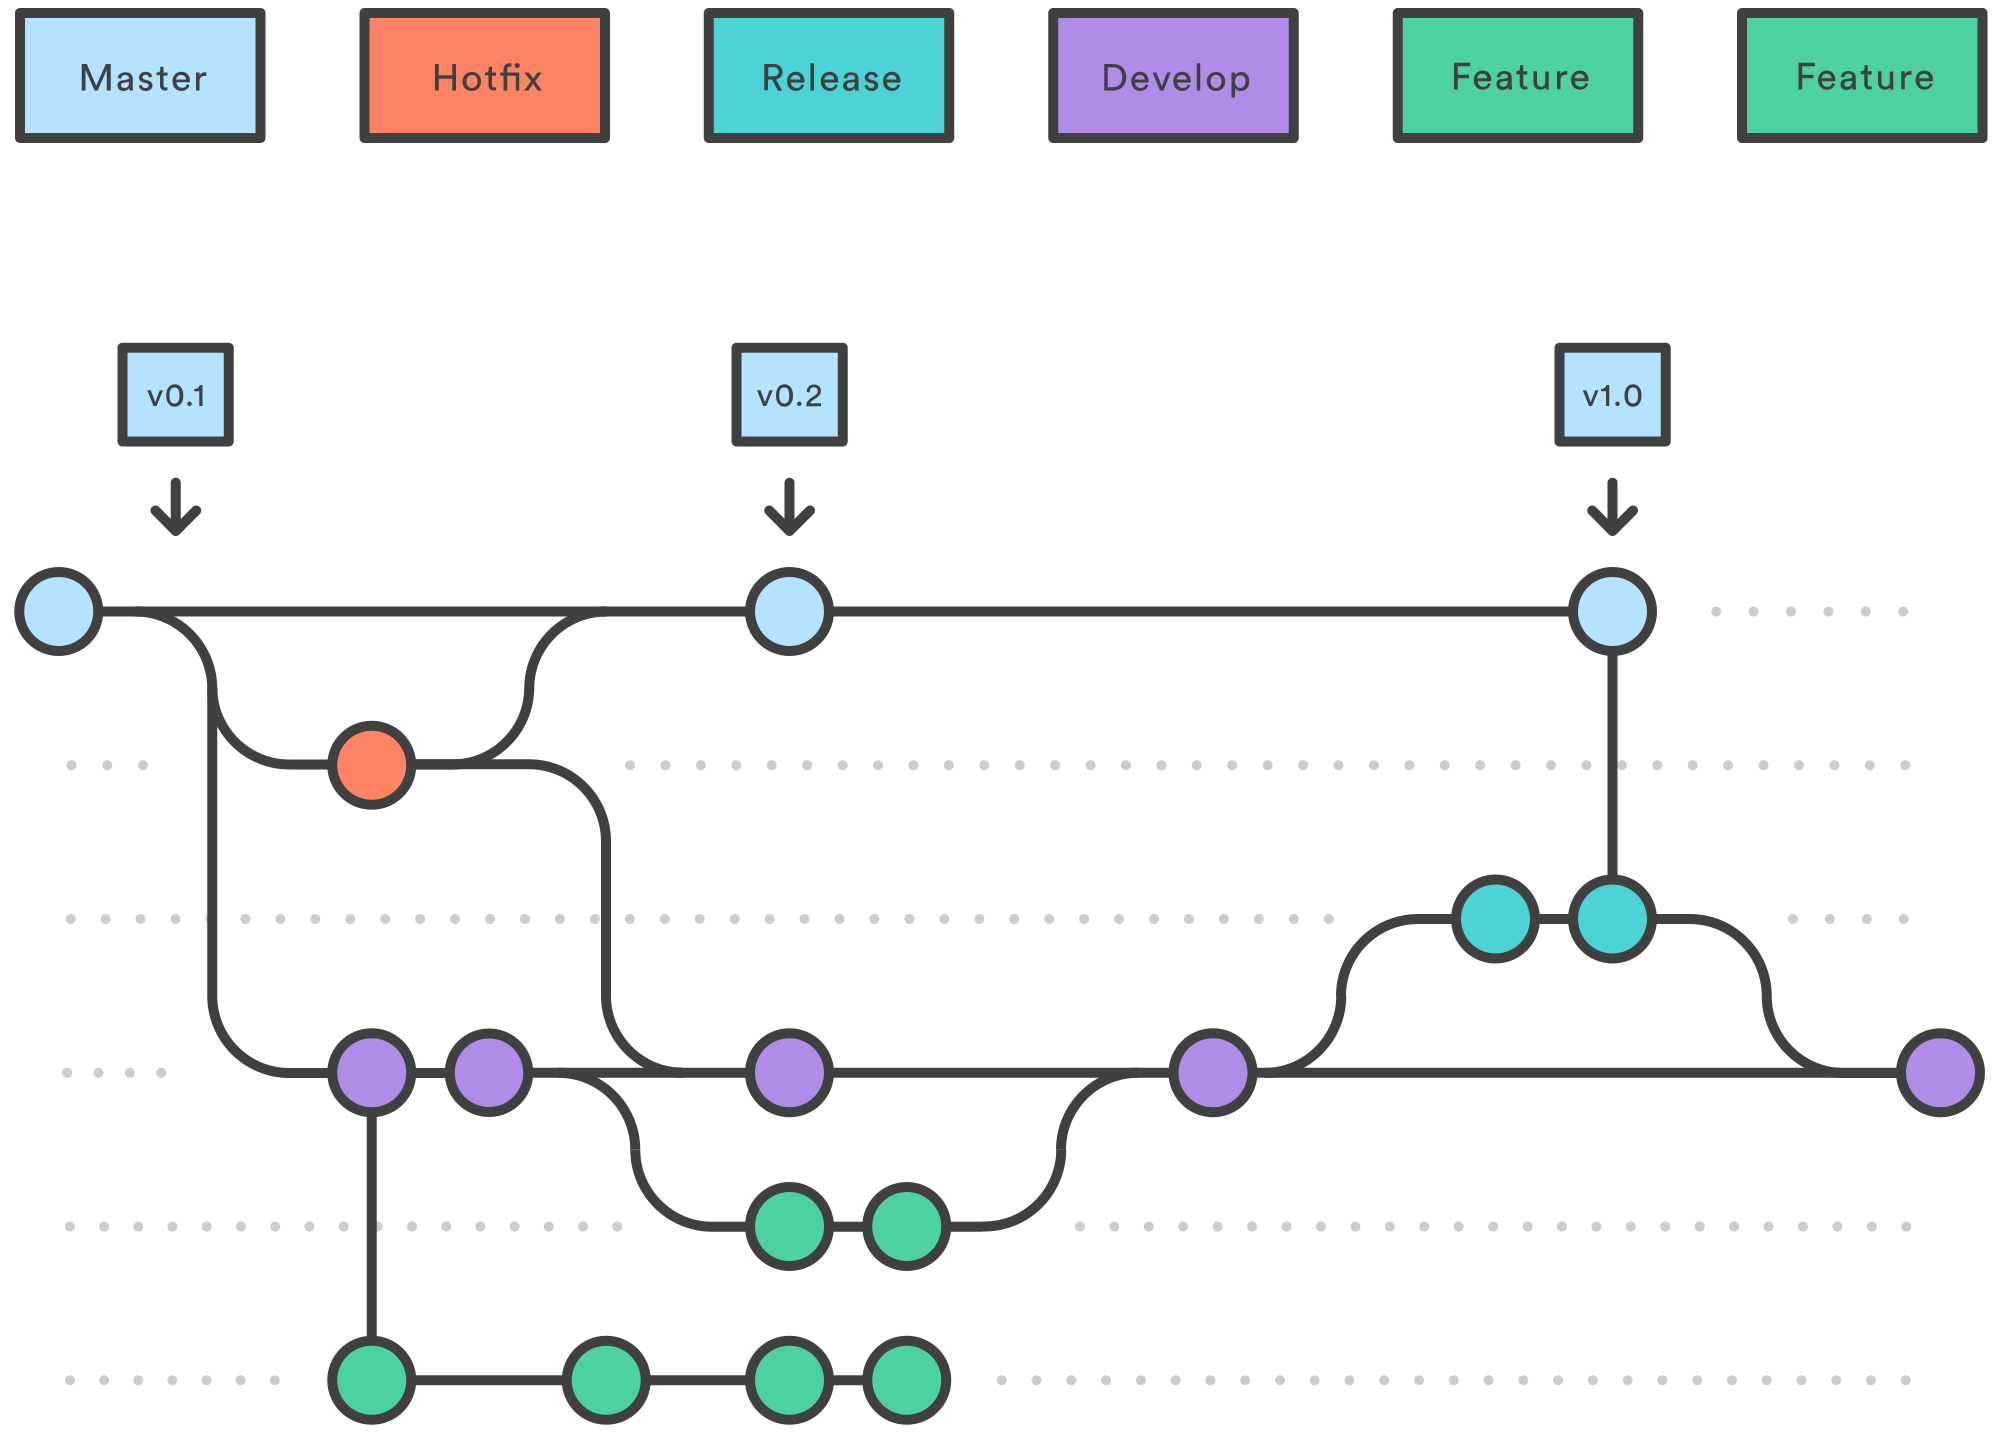
\includegraphics[width=\columnwidth]{img/gitflow}
	\caption[Gitflow]{Gitflow\footnotemark}
\end{figure}
\footnotetext{\cite{atlassian2020}}

Der Gitflow-Workflow definiert ein strenges Branching-Model und gibt jedem Typ von Branch (lediglich differenziert durch ihre Namen) eine spezifische Rolle. \code{Master} wird verwendet, um die Release-History festzuhalten. Hier finden sich Versionen des Projekts, die lauffähig sind und für sich alleine stehen (können). \code{Development} fungiert ähnlich wie \code{Master}, nur enthält es die gesamte Entwicklungshistorie des Projekts. Nun kommen die sogenannten \code{Feature}-Branches ins Spiel. Benannt werden Features hierarchisch. Im Projekt werden folgende zwei Gruppen verwendet: 

\begin{minipage}{\textwidth}
	\texttt{feature/\textbf{backend}/<konkretes-feature>}
	
	\texttt{feature/\textbf{frontend}/<konkretes-feature>}
\end{minipage}

Jedes Feature wird einem Verantwortlichen zugeteilt und wird meist auch von diesem bearbeitet. Sobald ein Feature fertig ist, wird es in \code{Development} zusammengeführt. Somit werden die Abstände zwischen Zusammenführungen verringert und der Arbeitsablauf wird einfacher. Schließlich gibt es auch noch einen Hotfix-Branch für dringende Änderungen.

Im Laufe der Entwicklung haben sich die Vorteile dieser Herangehensweise für das Team deutlich gezeigt. Unterschiedliche Features konnten, nachdem eine grundlegende Programmarchitektur umgesetzt worden ist, meist ohne Probleme zusammengeführt werden. 

\para{Nutzung von Stack für Notation [Schwenke]}

Der Taschenrechner soll als Eingabelogik für die Anwendung von Operationen die umgekehrte polnische Notation verwenden. Hierbei werden immer zunächst die Operanden und im Anschluss daran die darauf auszuführenden Operatoren angegeben. Dieser Ansatz ermöglicht eine stapelbasierte Abarbeitung. 

Stacks werden, wie von den meisten Programmiersprachen, auch in Java in der Standardbibliothek unterstützt. Mit dabei sind Methoden wie \code{push} (für das Ablegen eines Objekts auf dem Stapel), \code{pop} (für das Entfernen und die Wiedergabe eines Objekts auf dem Stapel), \code{peek} (für die Wiedergabe ohne Entfernen eines Objekts auf dem Stapel) und \code{empty} (für das Leeren des Stapels). 

Jedoch müssen hierbei die besonderen Anforderungen des Taschenrechners beachtet werden. Operanden können von gänzlich unterschiedlichem Typus sein, zum Beispiel eine einfache Dezimalzahl oder auch ein Tupel, und viele Operationen benötigen mehr als die ersten (maximal zwei) Operanden auf dem Stack. Möchte man Elemente vom Stapel entfernen, kann man \code{pop} mehrmals aufrufen. Aufwändiger hingegen wird es bei \code{peek}. Möchte man mehrere Elemente vom Stapel einsehen ohne diese zu entfernen, muss man bei der Arbeit mit dem vorhandenen Stack einen weiteren bereithalten, nur um zwischengespeicherte Elemente lagern zu können. Anders ist es nicht möglich \code{peek} auf mehrere Elemente gleichzeitig anzuwenden. Gerade das ist aber bei der App notwendig. Weitere Methoden, die bei der umgekehrten polnischen Notation oft benötigt werden, aber nicht implementiert sind, sind \code{reverse} (für die Vertauschung der ersten zwei Elemente auf dem Stack, was wichtig für nicht-kommutative Operationen ist), \code{rollUp} (das unterste Elemente wird an den ersten Platz geschoben, das erste Element an den zweiten Platz usw.) und \code{rollDown} (das unterste Elemente wird an den ersten Platz geschoben, das erste Element an den zweiten Platz usw.).

Aufgrund dessen soll für dieses Projekt ein eigener Stapel implementiert werden. Dieser soll die zuvor genannten Funktionen mit unterschiedlichen Parametertypen unterstützen. Dabei ist darauf zu achten, dass die Programmierung generisch erfolgt und das Stack nicht nur alle Typen von Operanden unterstützt, sondern auch für gänzlich andere Klassenbäume in der App verwendet werden kann.

\para{Ansatz der Kalkulationsorchestrierung [Schwenke]}

Die App soll den Umgang mit unterschiedlichen Operanden-Typen beherrschen. Die Addition zweier Matrizen funktioniert anders als die Addition von zwei einfachen Dezimalzahlen. Java verfügt nativ weder über die entsprechenden Operanden noch über die Methoden für die Kalkulation. Auch die ausgewählte Bibliothek ist nicht ohne weiteres in der Lage Operationen auf alle Kombinationen von Operanden im folgenden Format einheitlich anzuwenden:

\begin{figure}[bht]
	\begin{lstlisting}[caption=Konzept für Nutzung generischer Schnittstelle, label=list:konzept-fuer-nutzung-generischer-schnittstelle]
	Operation.mit(matrixOperand, dezimalOperand, dezimalOperand)
	\end{lstlisting}    
\end{figure}

Einheitlichkeit ist notwendig, damit im Frontend der Applikation keine Logik vorhanden sein muss, die entscheidet wie genau (auf Basis der Operanden-Typen) eine Operation umgesetzt wird. Deswegen muss eine einfache Schnittstelle entwickelt werden, die für den Nutzer nur zwei Drehschrauben bereitstellt. Dies ist zunächst die Auswahl der gewünschten Operation. Das kann z.B. das Symbol \code{+} als übliches Zeichen für Addition sein. Anschließend wird eine Reihe von Operanden übergeben. Dieser Aufruf sollte schließlich das Ergebnis in Form eines Operanden zurückgeben. Im Fall der Addition einer Matrix mit einer rationalen Zahl wäre dies wiederrum eine Matrix. Die korrekte Kalkulation soll also dynamisch bestimmt werden. Wichtig zu klären ist hier auch das Verhalten im Falle eines Fehlschlags. Nicht alle Kombinationen von Operanden können unterstützt werden. Die Verwendung von \textit{Optionals} (ein \code{Optional} ist ein Objekt, das man sich als Datenbehälter vorstellen kann, der entweder einen Wert enthält oder leer – aber nicht \code{null} sein kann) bietet sich hier zwar an, wird jedoch von Java in der verwendeten Android API-Version nicht unterstützt. Deswegen ist hier geplant sogenannte \textit{checked Exceptions} zu verwenden. Diese müssen bei der Verwendung explizit aufgefangen und weiterverarbeitet werden. Die Abbildung einer Operanden-Kombination auf die entsprechende konkrete Kalkulationsmethode muss dementsprechend zur Laufzeit des Programms erfolgen. Ein solches Mapping ist in Java nur mithilfe des Reflection-Pakets möglich. Reflektion ermöglicht den Einblick in ein Objekt (neben der Nutzung des Punkt-Operators) in eine Klasse. Zum Beispiel kann man eine Methode anhand einer Kombination von Parametertypen finden und aufrufen. Es ist geplant diesen Ansatz für die Orchestrierung der Kalkulationen in der App zu verwenden. Auch ist es nicht notwendig nur eine vordefinierte Anzahl an Argumente anzunehmen. So kann es sinnvoll sein, dass eine Methode zur Erstellung eines Tupels eine beliebige Anzahl an Operanden annimmt. Auch das lässt sich mit Reflektion umsetzen.

Der große Vorteil dabei ist, dass nirgendwo explizit in einer Abfrage entschieden werden muss, welche Kombination von Operanden an welche Methode weitergeleitet werden soll. Die Zuordnung erfolgt rein über die Deklaration der Parametertypen in der Methode selbst. Das macht das Ändern und Erweitern der Rechenfunktionalitäten einfach. Es muss lediglich die entsprechende Klasse herausgesucht und eine Methode im korrekten Format hinzugefügt werden. 

\para{Nutzung von Stack für Notation [Schwenke]}

Der Taschenrechner soll als Eingabelogik für die Anwendung von Operationen die umgekehrte polnische Notation verwenden. Hierbei werden immer zunächst die Operanden und im Anschluss daran die darauf auszuführenden Operatoren angegeben. Dieser Ansatz ermöglicht eine stapelbasierte Abarbeitung. 

Stacks werden, wie von den meisten Programmiersprachen, auch in Java in der Standardbibliothek unterstützt. Mit dabei sind Methoden wie \code{push} (für das Ablegen eines Objekts auf dem Stapel), \code{pop} (für das Entfernen und die Wiedergabe eines Objekts auf dem Stapel), \code{peek} (für die Wiedergabe ohne Entfernen eines Objekts auf dem Stapel) und \code{empty} (für das Leeren des Stapels). 

Jedoch müssen hierbei die besonderen Anforderungen des Taschenrechners beachtet werden. Operanden können von gänzlich unterschiedlichem Typus sein, zum Beispiel eine einfache Dezimalzahl oder auch ein Tupel, und viele Operationen benötigen mehr als die ersten (maximal zwei) Operanden auf dem Stack. Möchte man Elemente vom Stapel entfernen, kann man \code{pop} mehrmals aufrufen. Aufwändiger hingegen wird es bei \code{peek}. Möchte man mehrere Elemente vom Stapel einsehen ohne diese zu entfernen, muss man bei der Arbeit mit dem vorhandenen Stack einen weiteren bereithalten, nur um zwischengespeicherte Elemente lagern zu können. Anders ist es nicht möglich \code{peek} auf mehrere Elemente gleichzeitig anzuwenden. Gerade das ist aber bei der App notwendig. Weitere Methoden, die bei der umgekehrten polnischen Notation oft benötigt werden, aber nicht implementiert sind, sind \code{reverse} (für die Vertauschung der ersten zwei Elemente auf dem Stack, was wichtig für nicht-kommutative Operationen ist), \code{rollUp} (das unterste Elemente wird an den ersten Platz geschoben, das erste Element an den zweiten Platz usw.) und \code{rollDown} (das unterste Elemente wird an den ersten Platz geschoben, das erste Element an den zweiten Platz usw.).

Aufgrund dessen soll für dieses Projekt ein eigener Stapel implementiert werden. Dieser soll die zuvor genannten Funktionen mit unterschiedlichen Parametertypen unterstützen. Dabei ist darauf zu achten, dass die Programmierung generisch erfolgt und das Stack nicht nur alle Typen von Operanden unterstützt, sondern auch für gänzlich andere Klassenbäume in der App verwendet werden kann.

\para{Ansatz der Kalkulationsorchestrierung [Schwenke]}

Die App soll den Umgang mit unterschiedlichen Operanden-Typen beherrschen. Die Addition zweier Matrizen funktioniert anders als die Addition von zwei einfachen Dezimalzahlen. Java verfügt nativ weder über die entsprechenden Operanden noch über die Methoden für die Kalkulation. Auch die ausgewählte Bibliothek ist nicht ohne weiteres in der Lage Operationen auf alle Kombinationen von Operanden im folgenden Format einheitlich anzuwenden:

\begin{figure}[bht]
	\begin{lstlisting}[caption=Konzept für Nutzung generischer Schnittstelle, label=list:konzept-fuer-nutzung-generischer-schnittstelle]
	Operation.mit(matrixOperand, dezimalOperand, dezimalOperand)
	\end{lstlisting}    
\end{figure}

Einheitlichkeit ist notwendig, damit im Frontend der Applikation keine Logik vorhanden sein muss, die entscheidet wie genau (auf Basis der Operanden-Typen) eine Operation umgesetzt wird. Deswegen muss eine einfache Schnittstelle entwickelt werden, die für den Nutzer nur zwei Drehschrauben bereitstellt. Dies ist zunächst die Auswahl der gewünschten Operation. Das kann z.B. das Symbol \code{+} als übliches Zeichen für Addition sein. Anschließend wird eine Reihe von Operanden übergeben. Dieser Aufruf sollte schließlich das Ergebnis in Form eines Operanden zurückgeben. Im Fall der Addition einer Matrix mit einer rationalen Zahl wäre dies wiederrum eine Matrix. Die korrekte Kalkulation soll also dynamisch bestimmt werden. Wichtig zu klären ist hier auch das Verhalten im Falle eines Fehlschlags. Nicht alle Kombinationen von Operanden können unterstützt werden. Die Verwendung von \textit{Optionals} (ein \code{Optional} ist ein Objekt, das man sich als Datenbehälter vorstellen kann, der entweder einen Wert enthält oder leer – aber nicht \code{null} sein kann) bietet sich hier zwar an, wird jedoch von Java in der verwendeten Android API-Version nicht unterstützt. Deswegen ist hier geplant sogenannte \textit{checked Exceptions} zu verwenden. Diese müssen bei der Verwendung explizit aufgefangen und weiterverarbeitet werden. Die Abbildung einer Operanden-Kombination auf die entsprechende konkrete Kalkulationsmethode muss dementsprechend zur Laufzeit des Programms erfolgen. Ein solches Mapping ist in Java nur mithilfe des Reflection-Pakets möglich. Reflektion ermöglicht den Einblick in ein Objekt (neben der Nutzung des Punkt-Operators) in eine Klasse. Zum Beispiel kann man eine Methode anhand einer Kombination von Parametertypen finden und aufrufen. Es ist geplant diesen Ansatz für die Orchestrierung der Kalkulationen in der App zu verwenden. Auch ist es nicht notwendig nur eine vordefinierte Anzahl an Argumente anzunehmen. So kann es sinnvoll sein, dass eine Methode zur Erstellung eines Tupels eine beliebige Anzahl an Operanden annimmt. Auch das lässt sich mit Reflektion umsetzen.

Der große Vorteil dabei ist, dass nirgendwo explizit in einer Abfrage entschieden werden muss, welche Kombination von Operanden an welche Methode weitergeleitet werden soll. Die Zuordnung erfolgt rein über die Deklaration der Parametertypen in der Methode selbst. Das macht das Ändern und Erweitern der Rechenfunktionalitäten einfach. Es muss lediglich die entsprechende Klasse herausgesucht und eine Methode im korrekten Format hinzugefügt werden. 

Zu entscheiden ist ebenfalls, ob das Gros der Rechenmethoden innerhalb der jeweiligen Operanden-Klassen oder dedizierten Klassen für die Kalkulation angesiedelt sind. Die erste Option hat neben der stärkeren Objektorientierung den Vorteil, dass immer klar ist, dass eine Methode mit den übergebenen Argumenten auf dem jeweiligen Objekt ausgeführt wird. Andererseits erhöht dies die Komplexität der Operanden-Klassen deutlich. Unterstützt man wie geplant 5 bis 7 dedizierte Typen von Operanden und 10 Kalkulationsarten, muss jede Klasse potenziell dutzende Methoden für die Rechnung enthalten. Die andere, und bevorzugte Option, ist die Auslagerung der Kalkulationsmethoden in eigenständige Klassen. Dies reduziert zwar nicht die Anzahl benötigter Methoden, isoliert die Rechenlogik jedoch in Klassen. Innerhalb dieser Klassen wird prozedural programmiert.  Eine typische Charakteristik von Objekten und deren Methoden ist \textit{Mutability}. Eine Methode bekommt ein Objekt und kann dieses verändern. Dies kann Testen unter Umständen aufwändiger gestalten. Durch Isolierung der Rechnungen in eigenen Klassen kann hingegen sichergestellt werden, dass jede Methode \textit{immutable}, also unveränderlich, ist. Das macht das Schreiben von Tests einfach. In Java kann Immutability durch die Verwendung von Annotationen sichergestellt werden. 



